\newpage

\chapterimage{blue21.jpeg} % Imagen de encabezado de capítulo
\chapterspaceabove{6.75cm} % Espacio en blanco desde la parte superior de la página hasta el título del capítulo en las páginas del capítulo
\chapterspacebelow{7.25cm} % Cantidad de espacio en blanco vertical desde el margen superior hasta el comienzo del texto en las páginas de los capítulos

%------------------------------------------------

\chapter*{PREFACIO}

Se recalca que esta obra son notas del curso de Matemáticas Discretas, por lo que es probable que exista algún error ortográfico o matemático. Se recomienda consultar la bibliografía proporcionada al final de este trabajo. La presente obra consta de todo el contenido que adjudicó el Lic. Rubén Ramón Vargas Palomares, quien imparte clases en la Escuela Superior de Física y Matemáticas (ESFM) en el Instituto Politécnico Nacional (IPN). Hice el mayor esfuerzo en estructurar el libro a base de proposiciones, ejercicios, notas, etc.; y se agregaron y modificaron algunas definiciones, a fin de lograr una mayor comprensión sin llegar a tener alguna ambigüedad.\\


Cada capítulo contiene varios ejercicios y demostraciones. Estos son de diversos tipos y pueden ayudar a tener una mejor comprensión del tema. Cabe mencionar que este libro fue mecanografiado por Marco Antonio Molina Mendoza, estudiante de la Escuela Superior de Física y Matemáticas. Si lo deseas o lo requieres, puedes imprimir esta obra, eres libre de hacerlo y no necesitas autorización. Cualquier mención a esta obra es apreciada, pero no requerida. Se sigue trabajando para corregir errores y/o mejorar este trabajo, por lo que está en constante cambio. Se recomienda entrar en  \href{https://linktr.ee/biblioteca_esfm}{\textbf{\color{jblueleft}Biblioteca ESFM}} para encontrar la versión más actualizada.

\begin{center}
    \begin{tikzpicture}
        \node[fill=white] at (0,0) {\qrcode[hyperlink, height=3cm]{https://linktr.ee/biblioteca_esfm}};
    \end{tikzpicture}
\end{center}

Algunos cambios han sido resultado de los comentarios de mis amigos y estudiantes de la Escuela Superior de Física y Matemáticas. Estas son algunas de las muchas mejoras que se han incorporado en esta edición.
\begin{itemize}
    \item Aspecto estético mejorado: He trabajo arduamente para crear un diseño atractivo y cómodo a la vista. Nuevas fuentes, estilos y esquemas de color se han utilizado para mejorar la legibilidad y facilitar la asimilación de los conceptos.
    \item Errores ortográficos y matemáticos corregidos: He realizado una revisión minuciosa para garantizar la precisión en todos los aspectos del contenido. Los errores ortográficos y matemáticos se han corregido para ofrecer una experiencia de aprendizaje fluida y confiable.
    \item Imágenes actualizadas: He renovado todas las imágenes y gráficos del libro para asegurarme de que sean claros, informativos y visualmente atractivos. Las nuevas ilustraciones ayudarán a comprender mejor los conceptos y aplicaciones de la matemática discreta en el mundo real.
    \item Ejemplos adicionales y ejercicios prácticos: He añadido más ejemplos paso a paso y problemas resueltos para reforzar el entendimiento de los temas discutidos.
    %\item Recuadros de resumen y notas destacadas: Hemos agregado recuadros de resumen al final de cada sección para recapitular los puntos clave. Además, hemos incluido notas destacadas para enfatizar conceptos importantes y recordatorios útiles a lo largo del libro.
\end{itemize}

Con una presentación clara y concisa de los temas, busco fomentar la apreciación de la belleza y utilidad de esta rama de las matemáticas. Se aspira a que los lectores adquieran las habilidades y conocimientos necesarios para resolver problemas complejos y se sientan motivados a explorar aplicaciones más avanzadas de la matemática discreta en su futuro académico y profesional.\\


Este libro (en PDF) está diseñado en tres grandes enlaces
\begin{itemize}
    \item Números de páginas: Lo podrás encontrar en la parte superior derecha e izquierda dependiendo si es una página par o impar; al dar clic te llevará al índice de este libro.
    \item Nombres de secciones en el encabezado: Lo podrás encontrar en la parte superior derecha de cada página impar; al dar clic te llevará al comienzo de dicha sección.
    \item Nombres de capítulos en el encabezado: Lo podrás encontrar en la parte superior izquierda de cada página par; al dar clic te llevará al comienzo de dicho capítulo.
\end{itemize}

Esta obra se hizo gracias a \textbf{\textsf{\color{jblueleft}El Libro Azul}} (tercera versión), una plantilla hecha en \LaTeX\ que podrás encontrar en:
\begin{center}
    \color{jblueleft}
    \underline{\url{https://drive.google.com/drive/folders/1_zVKfxadoDAeL0Yrz9_RzXQuhQfiJ8ig}}
\end{center}
\cczero\ Esta plantilla se publica en el dominio público utilizando el código CC0. En la medida de lo posible bajo la ley, yo renunció a todos los derechos de autor y derechos relacionados o conexos a este trabajo.\\


Además, las imágenes que se presentan en este libro están hechas con el paquete \texttt{Tikz}, una herramienta para la producción de gráficos vectoriales. Dichas imágenes son de elaboración propia; y de igual manera, son de dominio público.

\vfill

\begin{center}
    \begin{tikzpicture}
        \node at (0,0) {
\includegraphics[width=3.5cm]{Images/ESCUDO_ESFM.pdf}};
        \node at (6,0) {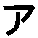
\includegraphics[width=3.5cm]{Images/LOGO.pdf}};
    \end{tikzpicture}
\end{center}